\documentclass[
nopagebreaks,
style=klope,
fleqn]{powerdot}
\usepackage{amsmath, amsfonts}
\usepackage{hyperref}
\usepackage{breakurl}
\usepackage{paralist}
\usepackage{subfig}
\usepackage{algpseudocode}
\usepackage{algorithmicx}
\usepackage{algorithm}
\title{K-Means Clustering on GPU}
\author{Yige Hu and Zhiting Zhu}
\date{}

\begin{document}

\maketitle

% declaration of the new block
\algblock{ParFor}{EndParFor}
% customizing the new block
\algnewcommand\algorithmicparfor{\textbf{parfor}}
\algnewcommand\algorithmicpardo{\textbf{do}}
\algnewcommand\algorithmicendparfor{\textbf{end\ parfor}}
\algrenewtext{ParFor}[1]{\algorithmicparfor\ #1\ \algorithmicpardo}
\algrenewtext{EndParFor}{\algorithmicendparfor}

\algnewcommand\algorithmicinput{\textbf{INPUT:}}
\algnewcommand\INPUT{\item[\algorithmicinput]}

\begin{slide} {Problem}
  \begin{compactitem}
  \item{Input: a set of data points $\{x_i|i = 1..n\} \subseteq
    \mathbb{R}^d $}
  \item{Task: partition the n data points
    in to k($\leq n$) sets S = $\{S_1, S_2, ..., S_k\}$ so as to minimize
    the within-cluster sum of squared
    errors, $$\arg\min_{S}\sum_{i=1}^{k}\sum_{x \in S_i} \parallel x -
    \mu(S_i)\parallel$$ where $\mu(S_i)$ is the mean of points in $S_i$}
  \item{NP-hard problem for global optimal solution
    \begin{compactitem}
    \item{In general d dimension Euclidean space even with 2 clusters~\cite{k-means-euclidean}}
    \item{k clusters in the same plane~\cite{k-means-plane}}
    \end{compactitem}
  }
  \item{Heuristic algorithm}
  \end{compactitem}
  \vspace{-0.6in}
  \begin{figure}
    \flushright
    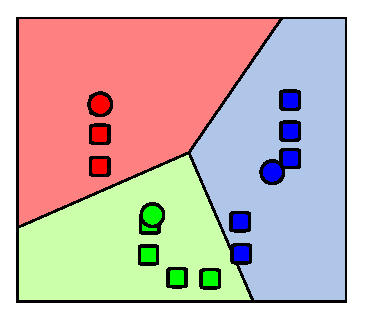
\includegraphics[scale=.5]{fig/K_Means_Example_Step_4.eps}
  \end{figure}
\end{slide}

\begin{slide} {Sequential Algorithm: example}
  \begin{figure}[h]
    \centering
    \subfloat[t][~\cite{f1}]{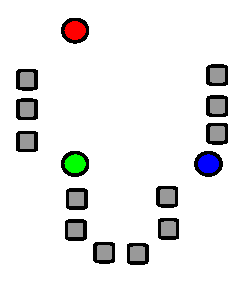
\includegraphics[scale=.5]{fig/K_Means_Example_Step_1.eps}}\qquad
    \subfloat[t][~\cite{f2}]{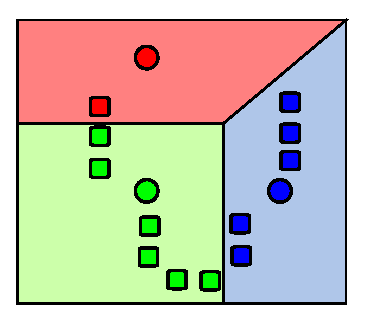
\includegraphics[scale=.5]{fig/K_Means_Example_Step_2.eps}}\\
    \subfloat[t][~\cite{f3}]{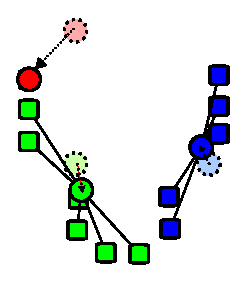
\includegraphics[scale=.5]{fig/K_Means_Example_Step_3.eps}}\qquad
    \subfloat[t][~\cite{f4}]{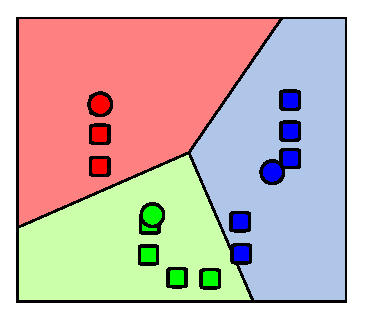
\includegraphics[scale=.5]{fig/K_Means_Example_Step_4.eps}}
  \end{figure}
  \begin{compactitem}
  \item{Problem size: $N$ $d$-dimensional data points, put into $K$ clusters.}
  \end{compactitem}
\end{slide}

\begin{slide} {Sequential Algorithm}
  \begin{algorithmic}[1]
    \INPUT $K$: Number of clusters; $N$: number of d-dimensional data points; $p$: data points. 
    \Function{seq\_k-means}{$p, N, K$}
    \State Randomly generate $K$ points as cluster centroids $c[]$
    \While {!termination\_condition }
    \State Assign each point to the nearest cluster centroid
    \State Recompute the new cluster centroids
    \EndWhile
    \EndFunction
  \end{algorithmic}
  \begin{compactitem}
    \vspace{.5in}
    \item{Suppose the algorithm runs m iterations. Time complexity: O(NKdm)}
  \end{compactitem}
\end{slide}

\begin{slide} {Parallel Algorithm}
  \footnotesize
  \begin{algorithmic}[1]
    \INPUT $K$: Number of clusters; $N$: number of d-dimensional data points; $p$: data points.
    \Function{par\_k-means}{$p, N, K$} \label{alg:p}
%    \State Partition N data objects evenly among all threads
    \State Randomly choose $K$ points as cluster centroids $c[]$
    \While {! termination\_condition}
    \ParFor {i = 1..N}
    \For {j = 1..K}
    \State Compute distance between point $p(i)$ and centroid $c(j)$
    \EndFor
    \State Find the nearest centroid $c_{nearest}$ for $p(i)$
    \State Change membership of $p(i)$ to the cluster with $c_{nearest}$
    \State Accumulate $p(i)$'s coordinates to the cluster's new centroid
    \EndParFor
    \State Compute new $c[]$: divide the accumulated coords by num\_points
    \State Recalculate termination condition
    \EndWhile
    \EndFunction  
  \end{algorithmic}
  \begin{compactitem}
    \vspace{5mm}
  \item{Suppose m iterations. 
    Work: O(NKdm), Depth: O(Kdm).}
  \end{compactitem}
\end{slide}

\begin{slide}{Goals and Challenges}
  \begin{compactitem}
    \item{CUDA implementation.}
    \item{GPU-related optimizations:}
    \begin{compactitem}
    \item{Control divergence;}
    \item{Coalesced memory access;}
    \item{Shared/constant memory usage}
    \item{etc...}
    \end{compactitem}
  \item{Limitation: GPU memory size.}
   \item{Problem size:}
     \begin{compactitem}
     \item{$\geq$ 600,000 points with $\geq$ 40 dimensions, $\geq$ 120 centroids;}
     \item{Efficient memory usage to increase solvable problem size.}
     \end{compactitem}
  \end{compactitem}
\end{slide}

\begin{slide} {References}
\footnotesize
\bibliographystyle{acm}
\bibliography{bibliography}
\end{slide}
\end{document}
